\section{Build structure}
\label{Sprint2_buildstructure}
\textit{This section describes the change made to the build structure of the apps and libraries in the project, in order to get a lower build time when building apps and libraries.}

\subsection{Motivation}

When the 2nd sprint started, the apps and libraries recursively downloaded and built all the libraries they were dependent on. This resulted in large repositories, since many libraries were included multiple times in one project. The graph in Figure \ref{oldbuild} shows the build tree for the sequence app. The darker circles are all local-db. As seen from the graph the library local-db is built 16 times before the sequence app itself is built. All in all the entire project for sequence had to build 31 libraries before it could build the app. Which took a lot of time on the build server.

\begin{figure}[H]
	\centering
	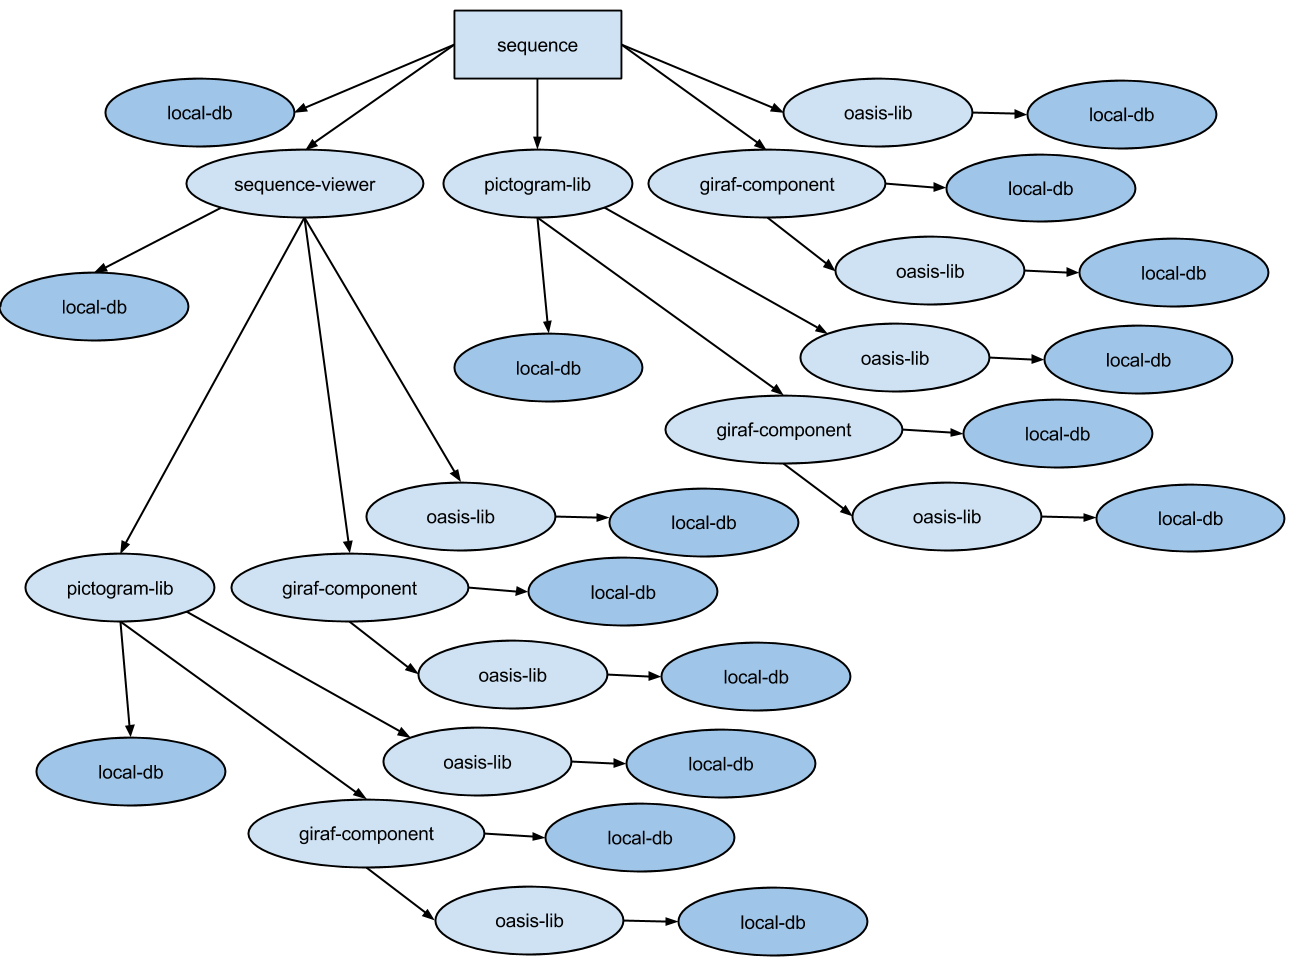
\includegraphics[width=0.8 \textwidth]{pictures/oldbuild.png}
	\caption{Build tree for sequence built recursively}
	\label{oldbuild}
\end{figure}

\subsection{Android archive}
As a solution, we wanted each library to build a library file, which could be used in multiple places. This would reduce the build time of all the projects since the apps or libraries would only need to download the pre-built library files.
This is where Android ARchive (AAR) files are introduced. AAR files are binary distributions of an Android Library Project, which works like a standard Java Archive (JAR) library. The difference between a JAR library and an AAR library is that the AAR library includes resources, such as images, which allows for visual components like a login screen, which can then be used across multiple apps.\\
Since more groups were involved in the reformation of the build structure, we refer to Section \ref{Collab_secBuildStructure} for the collaboration aspect.

\subsection{Solution}
By using a pre-built library, each app only has to build itself with the libraries included in the app as shown in the graph in Figure \ref{newbuild}. It is important to know that all libraries included in other libraries have to be included by the app. It means that even if sequence did not use dblib directly, it would still have to include it because ‘giraf-component’ is using it. This can be accomplished by using any tree traversal algorithm that returns all unique libraries in the tree from Figure \ref{oldbuild}.

\begin{figure}[H]
	\centering
	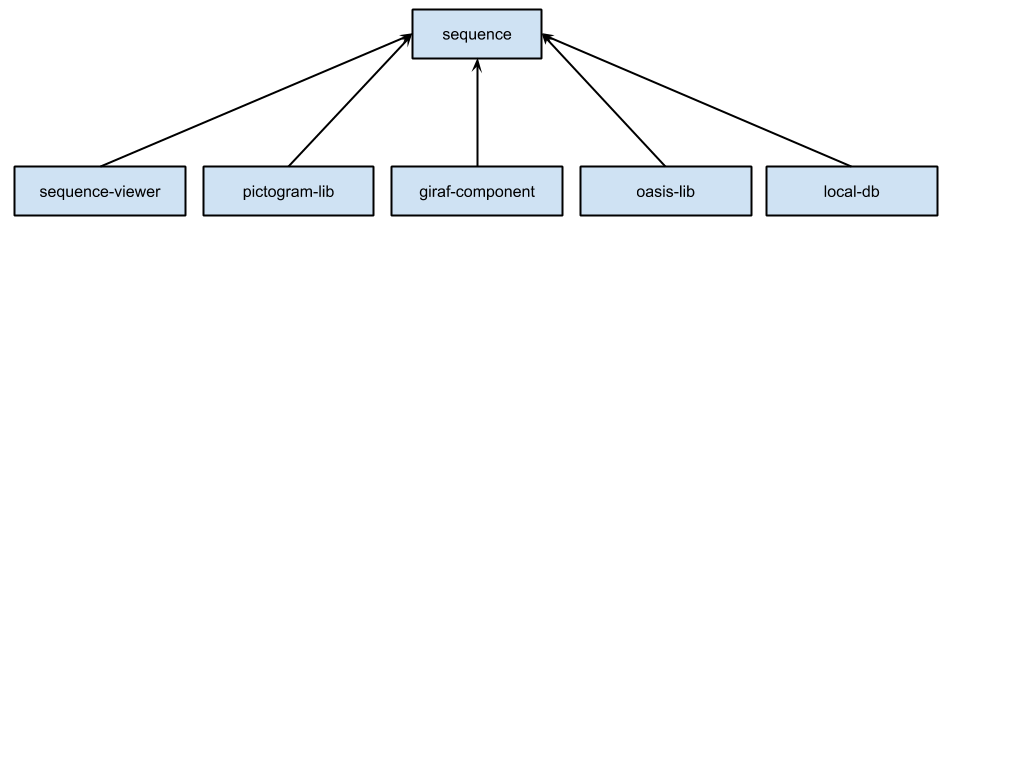
\includegraphics[width=0.8 \textwidth]{pictures/newbuild.png}
	\caption{Build tree for sequence built using AAR files}
	\label{newbuild}
\end{figure}

Before implementing this solution, libraries could be included once for every other library previously included in the app, and once for the app itself. This meant that if i.e sequence added the library sequence-viewer, then pictogram-lib, then giraf-component, then dblib, and then lastly local-db; then sequence-viewer would be added once, pictogram-lib twice, giraf-component four times, oasis-lib eight times, and ‘local-db sixteen times. This followed the arithmetic series:

\begin{center}
	$1 lib_{1} + 2 lib_{2} + 4 lib_{3} + 8 lib_{4} + 16 lib_{5} ... 2^{n-1} lib_{n} $	
\end{center}

This can be summarized to:
\begin{center}
    $\displaystyle\sum_{i=0}^{i<n} 2^i$
\end{center}

Where \textit{n} is the number of different libraries added to the app.

This was the worst case scenario but as it can be seen from Section \ref{Sprint2_SecDependencies} most apps were in a worst case state before the change.
After implementing the solution, the total number of library-builds were reduced to one for every different library. This meant that after the change there was a linear growth between the number of libraries and the number of library-builds.

As it can be seen from Table \ref{Table_BuildStructure_BeforeAfter}, our solution reduced the number of libraries being built drastically, which in turn reduced the build time for each app on Jenkins by a detectable margin.

\begin{table}[H]
	\centering
	\begin{tabularx}{\textwidth}{>{\raggedright}Xp{\textwidth/3}p{\textwidth/3}}
		 & \textbf{Builds Before} & \textbf{Builds After} \\ \noalign{\vskip 2mm}
		\hline \textbf{Launcher}: & 8 (barcodescanner is only built once) & 4 \\ \noalign{\vskip 2mm}
		\hline \textbf{Sequence}: & 31 & 5 \\ \noalign{\vskip 2mm}
		\hline \textbf{Timer}: & 18 (DrawLib, TimerLib, and wheel are only built once each) & 7 \\ \noalign{\vskip 2mm}
		\hline \textbf{Pictocreator}: & 15 & 4 \\ \noalign{\vskip 2mm}
		\hline \textbf{Categorymanager}: & 17 (category-lib and Ambilwarna are only built once each) & 6 \\ \noalign{\vskip 2mm}
		\hline \textbf{Pictosearch}: & 7 & 3 \\ \noalign{\vskip 2mm}
		\hline \textbf{Voicegame}: & 7 & 3 \\ \noalign{\vskip 2mm}
		\hline \textbf{Categorygame}: & 15 & 4 \\ \noalign{\vskip 2mm}
		\hline \textbf{Pictoreader}: & 17 (category-lib and Ambilwarna are only built once each) & 6 \\ \noalign{\vskip 2mm}
		\hline \textbf{Lifestory}: & 31 & 5 \\ \noalign{\vskip 2mm}
		\hline \textbf{Ugeplan}: & 15 & 4 \\ \noalign{\vskip 2mm}
		\hline \textbf{Administration}: & 7 & 3 \\ \noalign{\vskip 2mm}
		\hline
	\end{tabularx}
	\label{Table_BuildStructure_BeforeAfter}
	\caption{Number of builds before and after}
\end{table}
